\chapter{Geometrie des expandierenden Universums}

Im Mittelpunkt stehen das expandierende Universum und seine Geometrie. Ziel ist es, zu beschreiben, was es bedeutet, dass sich der Raum ausdehnt, bevor wir fragen, wodurch diese Expansion angetrieben wird. Die Newtonsche \(F=ma\) Kosmologie kommt später; erst danach werden Geometrie und Dynamik zum vollständigen Friedmann--Robertson--Walker-Rahmen zusammengeführt.

\section{Mitbewegte Koordinaten auf einer expandierenden Geraden}

Beginnen wir mit dem einfachstmöglichen Beispiel: einem eindimensionalen Raum, nicht der Raumzeit. Stellen wir uns eine unendliche Gerade mit gleichmäßig darauf verteilten Galaxien vor. Die Koordinate \(x\) misst noch keinen physikalischen Abstand. Sie bezeichnet die Galaxien. Man kann \(x\) als Namen einer Galaxie auffassen; dieser Name bleibt der Galaxie zugeordnet, selbst wenn sich die gesamte Anordnung ausdehnt oder zusammenzieht.

Der physikalische Abstand zwischen der mit \(x=0\) bezeichneten Galaxie und der mit \(x=1\) bezeichneten Galaxie sei \(a\). Dann ist der physikalische Abstand zwischen beliebigen zwei Galaxien
\begin{equation}
d=a\,\Delta x.
\end{equation}
Die Koordinatendifferenz \(\Delta x\) ist lediglich die Differenz der Bezeichnungen. Der Faktor \(a\) wandelt diese Differenz in einen tatsächlichen, mit Maßstäben gemessenen Abstand um.

Stellen wir uns nun vor, die Gerade sei ein elastischer Faden, der gedehnt wird. Die Bezeichnungen bleiben den Galaxien zugeordnet, doch der Abstand zwischen benachbarten Galaxien ändert sich mit der Zeit. Dieselbe Beziehung lautet nun
\begin{equation}
d(t)=a(t)\,\Delta x.
\end{equation}
In diesem Stadium bedeutet Homogenität schlicht, dass benachbarte Galaxien überall gleich weit voneinander entfernt sind, auch wenn sich dieser gemeinsame Abstand mit der Zeit ändern kann.

\section{Das Hubble-Gesetz und das Fehlen eines Zentrums}

Um die Relativgeschwindigkeit zweier fest gewählter Galaxien zu bestimmen, halten wir das Galaxienpaar fest, sodass sich \(\Delta x\) nicht mit der Zeit ändert. Durch Differenzieren erhalten wir
\begin{align}
\dot d &= \dot a\,\Delta x \\
       &= \frac{\dot a}{a}\,a\,\Delta x \\
       &= \frac{\dot a}{a}\,d.
\end{align}
Definieren wir
\begin{equation}
H(t)\equiv \frac{\dot a}{a},
\end{equation}
dann gilt
\begin{equation}
\dot d = H(t)\,d.
\end{equation}
Das ist das Hubble-Gesetz.

Die historische Bezeichnung ``Hubble-Konstante'' ist irreführend. Die Größe ist im Raum konstant, nicht in der Zeit. Zu einem gegebenen Zeitpunkt hat sie für alle Galaxien denselben Wert, ändert sich aber im Allgemeinen im Lauf der Entwicklung des Universums. Treffender ist die Bezeichnung Hubble-Parameter.

Das Gesetz besagt, dass weiter entfernte Galaxien sich schneller entfernen. Es zeichnet kein Zentrum aus. In der Argumentation wird weder \(x=0\) noch irgendein anderer Punkt besonders hervorgehoben. Jeder Beobachter sieht dieselbe Gesetzmäßigkeit. Das expandierende Universum dieses Modells ist daher keine Explosion an einem ausgezeichneten Ort.

Die Rotverschiebung kommt unmittelbar ins Spiel. Tauschen zwei Galaxien, die sich voneinander entfernen, Lichtsignale aus, so ist das empfangene Licht rotverschoben. Je größer die Fluchtgeschwindigkeit, desto größer die Rotverschiebung. Spektrallinien geben uns daher Aufschluss über Fluchtgeschwindigkeiten. Abstände sind schwieriger zu messen, und Hubbles frühe Schätzungen waren grob. Sein erstes Diagramm ergab keine perfekte Gerade, sondern eine verstreute Punktwolke mit großen Unsicherheiten. Dennoch hielt das geometrische Prinzip dem Rauschen stand: Die Fluchtgeschwindigkeit ist proportional zum Abstand.

\begin{classroomqa}
\audiencequestion{Bewegen sich weit genug voneinander entfernte Galaxien nach dem Hubble-Gesetz schneller als mit Lichtgeschwindigkeit?}\lecturetimestamp{00:20:23}
\lecturerresponse{Ja, in diesem Sinne der Flucht tun sie das. Was Sie sagen, ist richtig. Darauf kommen wir ganz bestimmt noch zurück. Das ist eine der wichtigsten Fragen.}
\end{classroomqa}

\section{Höhere Dimensionen, Isotropie und die Zeitabhängigkeit von \(a(t)\)}

Wenn weitere räumliche Dimensionen hinzukommen, ändert sich nichts Wesentliches. In zwei Dimensionen stellen wir uns ein quadratisches Gitter von Galaxien vor, bezeichnet durch \((x,y)\), in drei Dimensionen eines mit Bezeichnungen \((x,y,z)\). Auch diese Koordinaten sind mitbewegte Bezeichnungen. Sie bewegen sich mit den Galaxien, statt den physikalischen Abstand direkt zu messen.

Warum sollte der Abstand in \(x\)-Richtung derselbe sein wie in \(y\)-Richtung? Die Antwort ist eine Beobachtungsfrage. Wären Galaxien in einer Richtung systematisch dichter gedrängt als in einer anderen, sähe der Himmel in verschiedene Richtungen unterschiedlich aus. Auf hinreichend großen Skalen ist das nicht der Fall. Diese Richtungsunabhängigkeit ist Isotropie.

In zwei Dimensionen beträgt der Abstand zwischen zwei Galaxien
\begin{equation}
d=a\sqrt{(\Delta x)^2+(\Delta y)^2},
\end{equation}
und in drei Dimensionen
\begin{equation}
d=a\sqrt{(\Delta x)^2+(\Delta y)^2+(\Delta z)^2}.
\end{equation}
Für ein festes Galaxienpaar bleiben die Koordinatendifferenzen konstant. Erneutes Differenzieren ergibt daher
\begin{equation}
\dot d=\frac{\dot a}{a}\,d.
\end{equation}
Das Hubble-Gesetz bleibt unverändert.

Homogenität bedeutet Gleichheit von Ort zu Ort. Isotropie bedeutet Gleichheit in allen Richtungen. Auf kleinen Skalen gilt keines von beidem exakt. Ein Blick durch die Milchstraße unterscheidet sich von einem Blick senkrecht zu ihrer Ebene, und einzelne Galaxien sind auf kurzen Abständen nicht gleichmäßig verteilt. Mittelt man jedoch über viele Galaxien, erscheint das Universum auf großen Skalen näherungsweise überall und in jeder Richtung gleich.

\begin{classroomqa}
\audiencequestion{Wenn die Geschwindigkeit proportional zum Abstand ist und der Abstand zunimmt, muss sich dann ein festes Galaxienpaar immer schneller voneinander entfernen?}\lecturetimestamp{00:40:22}
\lecturerresponse{Nein. Das Hubble-Gesetz besagt, dass die Fluchtgeschwindigkeit zu einem gegebenen Zeitpunkt proportional zum Abstand ist. Für sich genommen sagt es nicht aus, ob die Geschwindigkeit eines festen Galaxienpaars im Lauf der Zeit zunimmt oder abnimmt. Das hängt von der genauen Zeitabhängigkeit von \(a(t)\) ab. Wenn \(a(t)\propto t\), entfernen sich benachbarte Galaxien mit konstanter Geschwindigkeit voneinander. Wenn \(a(t)\propto t^2\), nimmt die Fluchtgeschwindigkeit eines festen Paars mit der Zeit zu. Wenn \(a(t)\propto \log t\), nimmt sie mit der Zeit ab. Das Gesetz \(\dot d=(\dot a/a)d\) gilt als Funktion des Abstands immer; Beschleunigung und Verzögerung sind jedoch davon getrennte Fragen.}
\end{classroomqa}

Lange Zeit erwarteten Kosmologen, dass sich die Expansion des Universums verlangsamt, da die Gravitation eine anfängliche Expansion bremsen sollte, so wie sie einen nach oben geworfenen Körper abbremst. Hier geht es lediglich darum, dass das Hubble-Gesetz für sich genommen das Verhalten von \(\dot a\) oder \(\ddot a\) nicht festlegt.

\begin{classroomqa}
\audiencequestion{Wie legt man den Anfangswert des Skalenfaktors \(a\) fest?}\lecturetimestamp{00:46:18}
\lecturerresponse{Seine Gesamtnormierung ist willkürlich. Physikalisch entscheidend ist nicht der Zahlenwert von \(a\) für sich genommen, sondern wie er sich ändert. Definiert man einen anderen Skalenfaktor \(b=3a\), so gilt \(\dot b/b=\dot a/a\). Eine Reskalierung von \(a\) mit einer Konstanten ändert die Konvention oder die Einheiten, nicht aber den Hubble-Parameter.}
\end{classroomqa}

\section{Von der räumlichen Metrik zur Raumzeitmetrik}

Ersetzen wir nun \(\Delta x\) durch \(dx\). Der physikalische Abstand zwischen benachbarten Punkten ist
\begin{equation}
ds=a\,dx,
\end{equation}
also gilt
\begin{equation}
ds^2=a^2\,dx^2.
\end{equation}
Das ist die räumliche Metrik in einer Dimension. Der Koeffizient von \(dx^2\) ist
\begin{equation}
g_{xx}=a^2.
\end{equation}
Ein expandierendes Universum lässt sich somit dadurch beschreiben, dass der räumliche Teil der Metrik von der Zeit abhängt.

Um vom Raum zur Raumzeit überzugehen, verwenden wir das relativistische Linienelement. In einer räumlichen Dimension gilt
\begin{equation}
d\tau^2=dt^2-a^2(t)\,dx^2.
\end{equation}
Für einen mitbewegten Beobachter ist \(dx=0\), also \(d\tau=dt\). Die gewöhnliche kosmische Zeit ist die Eigenzeit, die von Uhren gemessen wird, welche sich mit den Galaxien bewegen.

Die Tafelzeichnung ist an dieser Stelle hilfreich, weil sie die mitbewegten Weltlinien, das Linienelement und die Metrikschreibweise zusammenführt.
\begin{figure}[H]
\centering
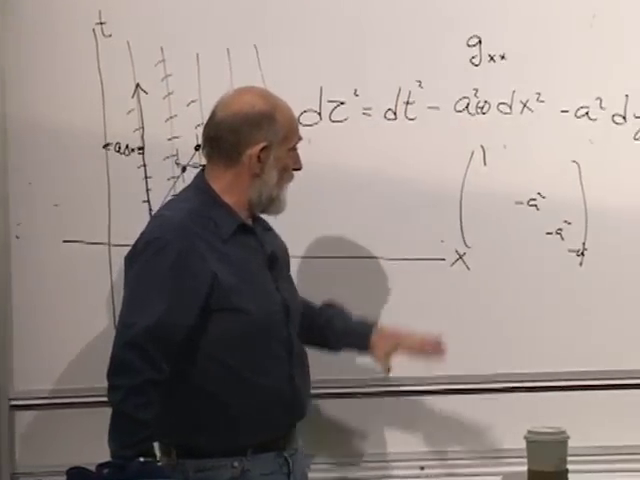
\includegraphics[width=0.82\textwidth]{lecture_01_figure_02.png}
\caption{Mitbewegte Weltlinien in einem expandierenden eindimensionalen Universum und das zugehörige Raumzeitintervall.}
\end{figure}

In drei räumlichen Dimensionen ergibt dasselbe Schema die vorsichtige Verallgemeinerung\footnote{Die Tafel ist teilweise verdeckt, und zwar im Bereich 00:56:38--00:58:51. Diese dreidimensionale Form folgt der mündlichen Verallgemeinerung von einer auf drei räumliche Dimensionen sowie dem sichtbaren diagonalen Muster auf der Tafel.}
\begin{equation}
d\tau^2=dt^2-a^2(t)\bigl(dx^2+dy^2+dz^2\bigr),
\end{equation}
mit der Diagonalmetrik
\begin{equation}
g_{\mu\nu}=\mathrm{diag}\bigl(1,-a^2,-a^2,-a^2\bigr).
\end{equation}
Die gemischten Terme verschwinden:
\begin{equation}
g_{tx}=g_{ty}=g_{tz}=0.
\end{equation}

Homogenität bedeutet, dass die Metrikkoeffizienten zwar von der Zeit, nicht aber vom Ort abhängen dürfen. Isotropie bedeutet, dass die drei räumlichen Richtungen auf dieselbe Weise eingehen.

\begin{classroomqa}
\audiencequestion{Sollen wir \(dx\) nicht als Abstand auffassen?}\lecturetimestamp{01:01:18}
\lecturerresponse{Nein. \(dx\) ist nicht der Abstand. \(a\,dx\) ist der Abstand. \(dx\) ist lediglich ein Koordinatenintervall. Man kann es sich so vorstellen: Zu einem bestimmten Zeitpunkt zeichnet jemand ein Koordinatennetz durch die Galaxien und sorgt dann dafür, dass das Netz ihnen folgt. Der Koordinatenabstand bleibt konstruktionsbedingt konstant, während sich der physikalische Abstand ändert. Man könnte die Längeneinheiten statt in \(a\) auch in \(x\) unterbringen; das ist eine Konvention. Entscheidend ist das Produkt \(a\,dx\).}
\end{classroomqa}

\begin{classroomqa}
\audiencequestion{Der Metrikkoeffizient von \(dt^2\) ist gleich \(1\). Ist auch das nur eine Konvention?}\lecturetimestamp{01:03:24}
\lecturerresponse{Ja. Für sich genommen steckt darin keine Physik. Hinge der Koeffizient nur von der Zeit ab, könnte man die Zeitvariable so ändern, dass er einfach \(dt^2\) wäre. Ebenso kann man Einheiten mit \(c=1\) wählen. Keine Konvention ist hier hingegen, dass der Koeffizient nicht vom Ort abhängt, auch wenn er von der Zeit abhängen kann.}
\end{classroomqa}

\begin{classroomqa}
\audiencequestion{Was ergibt sich für den Energie-Impuls-Tensor, wenn man dies in Einsteins Feldgleichungen einsetzt?}\lecturetimestamp{01:05:59}
\lecturerresponse{Das ist die nächste Art von Frage, gehört aber zur Dynamik und nicht zur gegenwärtigen Diskussion. Man kann diese Metrik in Einsteins Gleichungen einsetzen und fragen, welche Energie-Impuls-Verteilung sie zu einer Lösung machen würde. Das ist sehr wichtig, doch im Moment geht es um Geometrie, nicht um Dynamik.}
\end{classroomqa}

\section{Was der Horizont verbirgt}

Das Universum wird auf großen Skalen nur näherungsweise als homogen und isotrop behandelt. Auf der Skala von Sternen, Planeten oder auch einzelnen Galaxien ist es keineswegs homogen. Auch bei lokalen Beobachtungen ist es nicht exakt isotrop.

Ein Feld eines Bauern veranschaulicht die Abhängigkeit von der Skala. Auf einer Skala wirkt es regelmäßig; auf einer viel kleineren Skala ist das offensichtlich nicht der Fall; auf einer Skala, die größer ist als das ganze Feld, wirkt es wiederum nicht mehr homogen. In der Kosmologie ist es ähnlich. Mittelt man über viele Galaxien, erscheint die Verteilung auf großen Skalen ungefähr gleichmäßig. Auf hinreichend kleinen Skalen ist sie es nicht.

Das Universum ist größer als der Teil, den wir sehen können, und größer als der Teil, den wir jemals sehen können. Auf den Skalen, die tatsächlich beobachtbar sind, ist es abgesehen von lokalen Schwankungen isotrop und homogen. Jenseits davon gibt es keine unmittelbare Beobachtungsgarantie.

\begin{classroomqa}
\audiencequestion{Sie sagten, wir würden es nie wirklich direkt herausfinden. Heißt das, dass es vielleicht einen indirekten Weg gibt, es herauszufinden?}\lecturetimestamp{01:10:34}
\lecturerresponse{Vielleicht. Heute geht man meist davon aus, dass das Universum auf hinreichend großen Skalen nicht homogen ist, und ich selbst vermute das auch. Doch diese Vermutung kann ich weder bestätigt bekommen noch widerlegt sehen, denn aus grundlegenden Gründen werden wir nicht viel weiter blicken können als heute. Das liegt an der Existenz eines Horizonts.}
\end{classroomqa}

\begin{classroomqa}
\audiencequestion{Könnte man nicht die Gravitation nutzen, um nach Massen jenseits dessen zu suchen, was man sehen kann?}\lecturetimestamp{01:11:53}
\lecturerresponse{Nein. Eine weit entfernte Masse kann uns einfach in den freien Fall versetzen. In einem geschlossenen Raum befinden wir uns im Gravitationsfeld der Sonne und umkreisen sie. Doch ohne nach draußen zu sehen, gibt es keine einfache Möglichkeit zu erkennen, dass die Sonne da ist. Nur Gezeitenkräfte verraten es; ist die Quelle weit genug entfernt, können diese Gezeiteneffekte zu klein sein, um nachweisbar zu sein.}
\end{classroomqa}

Der Horizont ist somit eine unüberwindbare Grenze für unmittelbare Erkenntnis. Er sagt sogar mit praktisch völliger Gewissheit, dass das Universum ein mindestens tausendmal größeres Volumen hat als der Bereich, den wir jemals sehen können, und verschiebt die Begründung dieser Behauptung auf später.

\section{Begrenzt, aber ohne Rand}

Wenden wir uns nun geschlossenen Geometrien zu. Die unendliche Gerade ist offen und unbegrenzt. Eine Strecke ist insofern begrenzt, als sie nur eine endliche Ausdehnung hat. Begrenzt bedeutet nicht, dass es einen Rand gibt, sondern dass die Ausdehnung endlich ist.

Ein Würfel mit Wänden eignet sich nicht. Er verletzt die Homogenität, denn jemand in Wandnähe ist nicht gleichwertig mit jemandem weit von einer Wand entfernt. Zudem verletzt er die Isotropie, denn selbst jemand im Zentrum sieht in verschiedene Richtungen Unterschiedliches.

Auch das Innere eines Kreises oder einer Kugel eignet sich nicht. Jemand im Zentrum sieht in alle Richtungen dasselbe, doch diese Symmetrie gilt nur für einen einzigen ausgezeichneten Punkt. Bewegt man sich vom Zentrum weg, ist die Wand in einer Richtung nah und in einer anderen weit entfernt. Für beliebige Beobachter ist der Raum dann weder homogen noch isotrop.

Auf sehr großen Skalen lautet die Arbeitshypothese, dass das Universum homogen und isotrop ist. Das ist das kosmologische Prinzip. Es ist nützlich, aber nicht vor Revision geschützt.

\begin{classroomqa}
\audiencequestion{Folgt aus Isotropie überall auch Homogenität?}\lecturetimestamp{01:18:57}
\lecturerresponse{Ja. Wenn jeder Beobachter in alle Richtungen dasselbe sieht, folgt daraus Homogenität. Die Umkehrung gilt jedoch nicht. Homogenität allein bedeutet nicht Isotropie. Ein Universum kann homogen sein und dennoch eine ausgezeichnete Richtung haben, etwa wenn es von Pfeilen erfüllt wäre, die alle in dieselbe Richtung zeigen.}
\end{classroomqa}

Das passende begrenzte Modell ist die Oberfläche einer strukturfreien Kugel. Ein zweidimensionales Wesen, das auf diese Oberfläche beschränkt ist, findet jeden Ort lokal wie jeden anderen und jede Richtung wie jede andere, obwohl seine Welt endlich ist. Sie ist begrenzt, aber ohne Rand.

\section{Ein geschlossenes eindimensionales Universum auf einem Kreis}

Um die Algebra einfach zu halten, reduzieren wir das Kugelbeispiel auf eine räumliche Dimension: Leben auf einem Kreis. In einer Dimension bedeutet Isotropie, dass links und rechts gleichwertig sind. Ein Kreis weist genau diese Eigenschaft auf. Wir wählen einen Punkt und nennen ihn \(\theta=0\). Jeder andere Punkt wird durch eine Winkelkoordinate \(\theta\) bezeichnet, gemessen im Bogenmaß. Ein Punkt unmittelbar auf einer Seite des Ursprungs lässt sich entweder durch einen kleinen negativen Winkel oder durch einen Winkel knapp unter \(2\pi\) beschreiben. Diese Periodizität gehört zur Geometrie.

Den Bewohnern des Kreises steht der Umfang zur Verfügung, nicht aber ein äußerer Radius oder ein Zentrum. Sie können die gesamte Strecke ringsum messen, indem sie am Kreis entlanggehen, bis sie zum selben Punkt zurückkehren. Zeichnet man den Kreis in einer umgebenden Ebene, kann man auch eine radiusähnliche Größe einführen. Sie gehört jedoch zur Einbettung und nicht zu der intrinsischen Geometrie, die die Bewohner messen.

Die Tafelzeichnung ist hier hilfreich, weil sie die Winkelbezeichnungen und den Gesamtumfang in derselben Darstellung zeigt.
\begin{figure}[H]
\centering
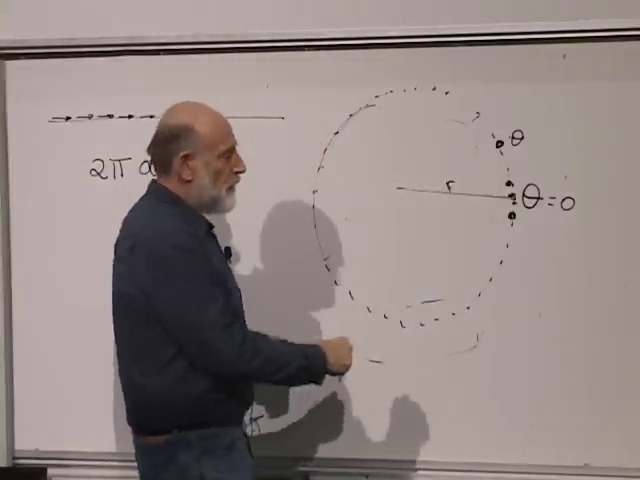
\includegraphics[width=0.82\textwidth]{lecture_01_figure_03.png}
\caption{Winkeldarstellung eines geschlossenen eindimensionalen Universums mit dem Gesamtumfang \(2\pi a\).}
\end{figure}

Eine praktische Konvention lautet\footnote{Zwischen 01:26:40--01:29:20 wechselt die Schreibweise kurz zwischen dem Gesamtumfang selbst als Skalenfaktor und der Darstellung als \(2\pi a\). Hier verwenden wir die spätere Konvention, weil sie in die Formel für die Bogenlänge übernommen wird.}
\begin{equation}
L=2\pi a,
\end{equation}
wobei \(L\) der Gesamtumfang ist.

Für einen kleinen Winkelabstand \(\Delta\theta\) ist der physikalische Abstand
\begin{equation}
d=a\,\Delta\theta.
\end{equation}
Im Grenzfall infinitesimaler Abstände erhalten wir
\begin{equation}
ds=a\,d\theta,
\end{equation}
und somit
\begin{equation}
ds^2=a^2\,d\theta^2.
\end{equation}
Das ist die lokale Metrik auf dem Kreis.

Hängt \(a\) von der Zeit ab, expandiert oder kontrahiert das geschlossene eindimensionale Universum. Für ein festes Galaxienpaar gilt
\begin{equation}
d(t)=a(t)\,\Delta\theta,
\end{equation}
also
\begin{equation}
\dot d=\dot a\,\Delta\theta
      =\frac{\dot a}{a}\,d.
\end{equation}
Auch hier gilt das Hubble-Gesetz, zumindest für Galaxienpaare, die nicht so weit voneinander entfernt sind, dass die andere Richtung um den Kreis herum mehrdeutig wird.

Die Raumzeitmetrik lautet dann
\begin{equation}
d\tau^2=dt^2-a^2(t)\,d\theta^2.
\end{equation}
Ist \(a\) konstant, ist das Raumzeitbild ein Zylinder. Gilt \(a\propto t\), ist es ein Kegel. Ändert sich \(a(t)\) unregelmäßiger, wird das Bild vasenförmig.

Lässt man das Bild rückwärts ablaufen, kommen sich die Galaxien immer näher. Gäbe es \(360\) Galaxien auf dem Kreis, wären sie zu späten Zeiten weit voneinander entfernt, zu früheren Zeiten sehr dicht beieinander und noch früher dichter zusammengedrängt. Schließlich wären sie keine getrennten Galaxien mehr und noch früher nicht einmal getrennte Atome. Dennoch gibt es weiterhin keinen ausgezeichneten Punkt im Raum.

Das ist die klarste Antwort auf die Frage, wo der Urknall in diesem Modell stattgefunden hat. Wenn \(a(t)\to 0\), geht jeder Abstand \(a(t)\,\Delta\theta\) gegen null. Das gesamte Universum schrumpft überall gleichzeitig. Die Galaxien fliegen nicht von einem ausgezeichneten Ort in einem äußeren Raum fort. Vielmehr ändert die Geometrie selbst ihren Maßstab. In diesem Sinn lautet die Antwort: überall.

\begin{classroomqa}
\audiencequestion{Sie sagten, die Raumzeit sei gekrümmt. Wäre sie auch gekrümmt, wenn sie ein Zylinder wäre?}\lecturetimestamp{01:38:04}
\lecturerresponse{Nein. Wäre sie ein Zylinder, wäre sie nicht gekrümmt. Das ist der Fall, in dem \(a\) zeitlich konstant ist. Gekrümmt wirkt der Zylinder nur, weil er in einem höherdimensionalen Raum gezeichnet wird. Schneidet man ihn auf, lässt er sich ohne Dehnung flach ausbreiten.}
\end{classroomqa}

Von dort führt die Diskussion zum Kegel. Wenn \(a\propto t\), ist das Raumzeitbild ein Kegel. Abseits seiner Spitze ist auch der Kegel im selben intrinsischen Sinn flach: Er lässt sich zu einer Ebene aufklappen. Die Spitze ist anders. Sie ist eine Kegelsingularität.

Als Nächstes folgen die Geometrie des sphärischen Universums und dann die Dynamik, die bestimmt, wie \(a(t)\) wächst oder schrumpft.
